\documentclass{article}
\usepackage{tikz}
\usetikzlibrary{shapes.geometric, arrows.meta, positioning}

% 定义样式
\tikzset{
    startstop/.style={
        draw, rectangle, rounded corners, minimum width=2.5cm, minimum height=1cm, align=center, fill=white, text=black, font=\rmfamily
    },
    process/.style={
        draw, rectangle, minimum width=3cm, minimum height=1cm, align=center, fill=white, text=black, text width=7cm, font=\rmfamily
    },
    input/.style={ 
        draw, trapezium, trapezium left angle=70, trapezium right angle=110, minimum width=2cm, minimum height=1cm, align=center, fill=white, text=black, text width=4cm, font=\rmfamily
    },
    decision/.style={
        draw, diamond, aspect=2, minimum width=3cm, minimum height=1cm, align=center, fill=yellow!30, text=black, font=\rmfamily
    },
    arrow/.style={
        thick,->,>=stealth
    },
    every node/.style={font=\rmfamily}
}

\begin{document}

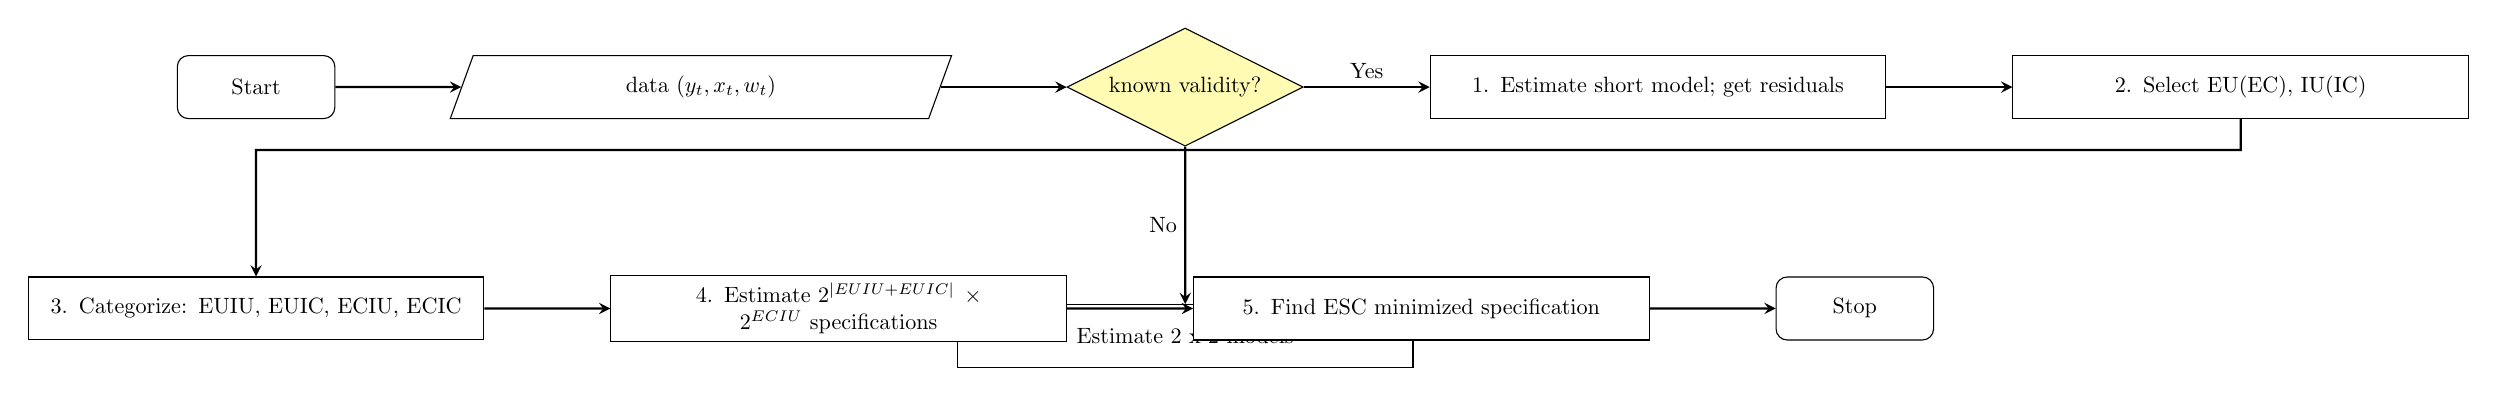
\begin{tikzpicture}[node distance=2.5cm and 2cm, auto, scale=0.8, transform shape]  % scale the entire drawing

    % 节点
    \node (start) [startstop] {Start};
    \node (input1) [input, right=of start] {data $(y_t,x_t,w_t)$};
    \node (validity) [decision, right=of input1] {known validity?};
    \node (estimate_short) [process, right=of validity] {1. Estimate short model; get residuals};
    \node (new_estimate) [process, below=of validity] {Estimate 2 x 2 models};
    \node (select) [process, right=of estimate_short] {2. Select EU(EC), IU(IC)};
    \node (categorize) [process, below=of start] {3. Categorize: EUIU, EUIC, ECIU, ECIC};
    \node (estimate) [process, right=of categorize] {4. Estimate $2^{|EUIU+EUIC|}\times 2^{ECIU}$ specifications};
    \node (find) [process, right=of estimate] {5. Find ESC minimized specification};
    \node (stop) [startstop, right=of find] {Stop};

    % 箭头
    \draw [arrow] (start) -- (input1);
    \draw [arrow] (input1) -- (validity);
    \draw [arrow] (validity) -- node[above] {Yes} (estimate_short);
    \draw [arrow] (validity) -- node[left] {No} (new_estimate);
    \draw [arrow] (estimate_short) -- (select);
    \draw [arrow] (select) -- ++(0,-1) -| (categorize);
    \draw [arrow] (categorize) -- (estimate);
    \draw [arrow] (estimate) -- (find);
    \draw [arrow] (find) -- (stop);

\end{tikzpicture}

\end{document}
